\newcommand{\webscaleoutfig}{
    \begin{figure}[tb]
    \centering
    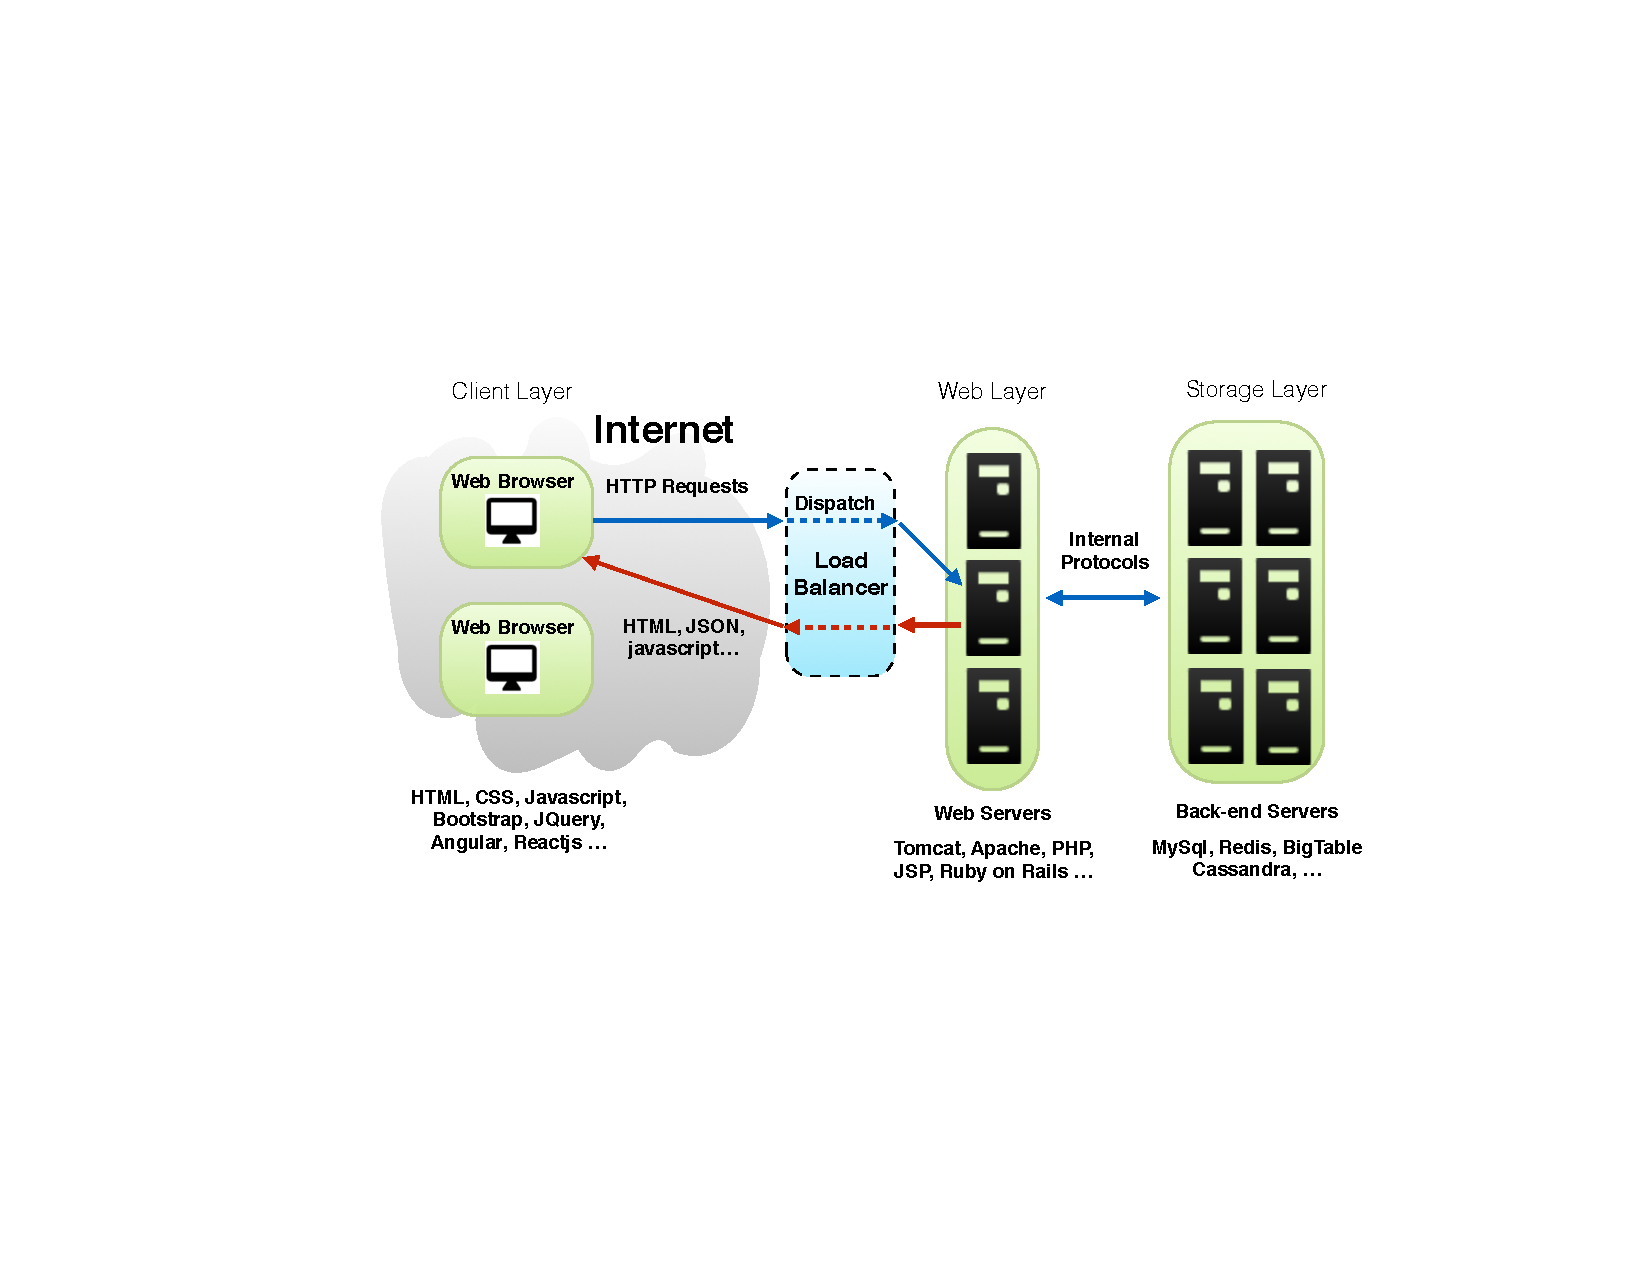
\includegraphics[width=\textwidth]{../figs/web_scale_out}
    \caption{Scalable design of multitier applications}
    \label{fig:webscaleout}
    \end{figure}
}

\newcommand{\architectureoverview}{
    \begin{figure*}[ht]
    \centering
    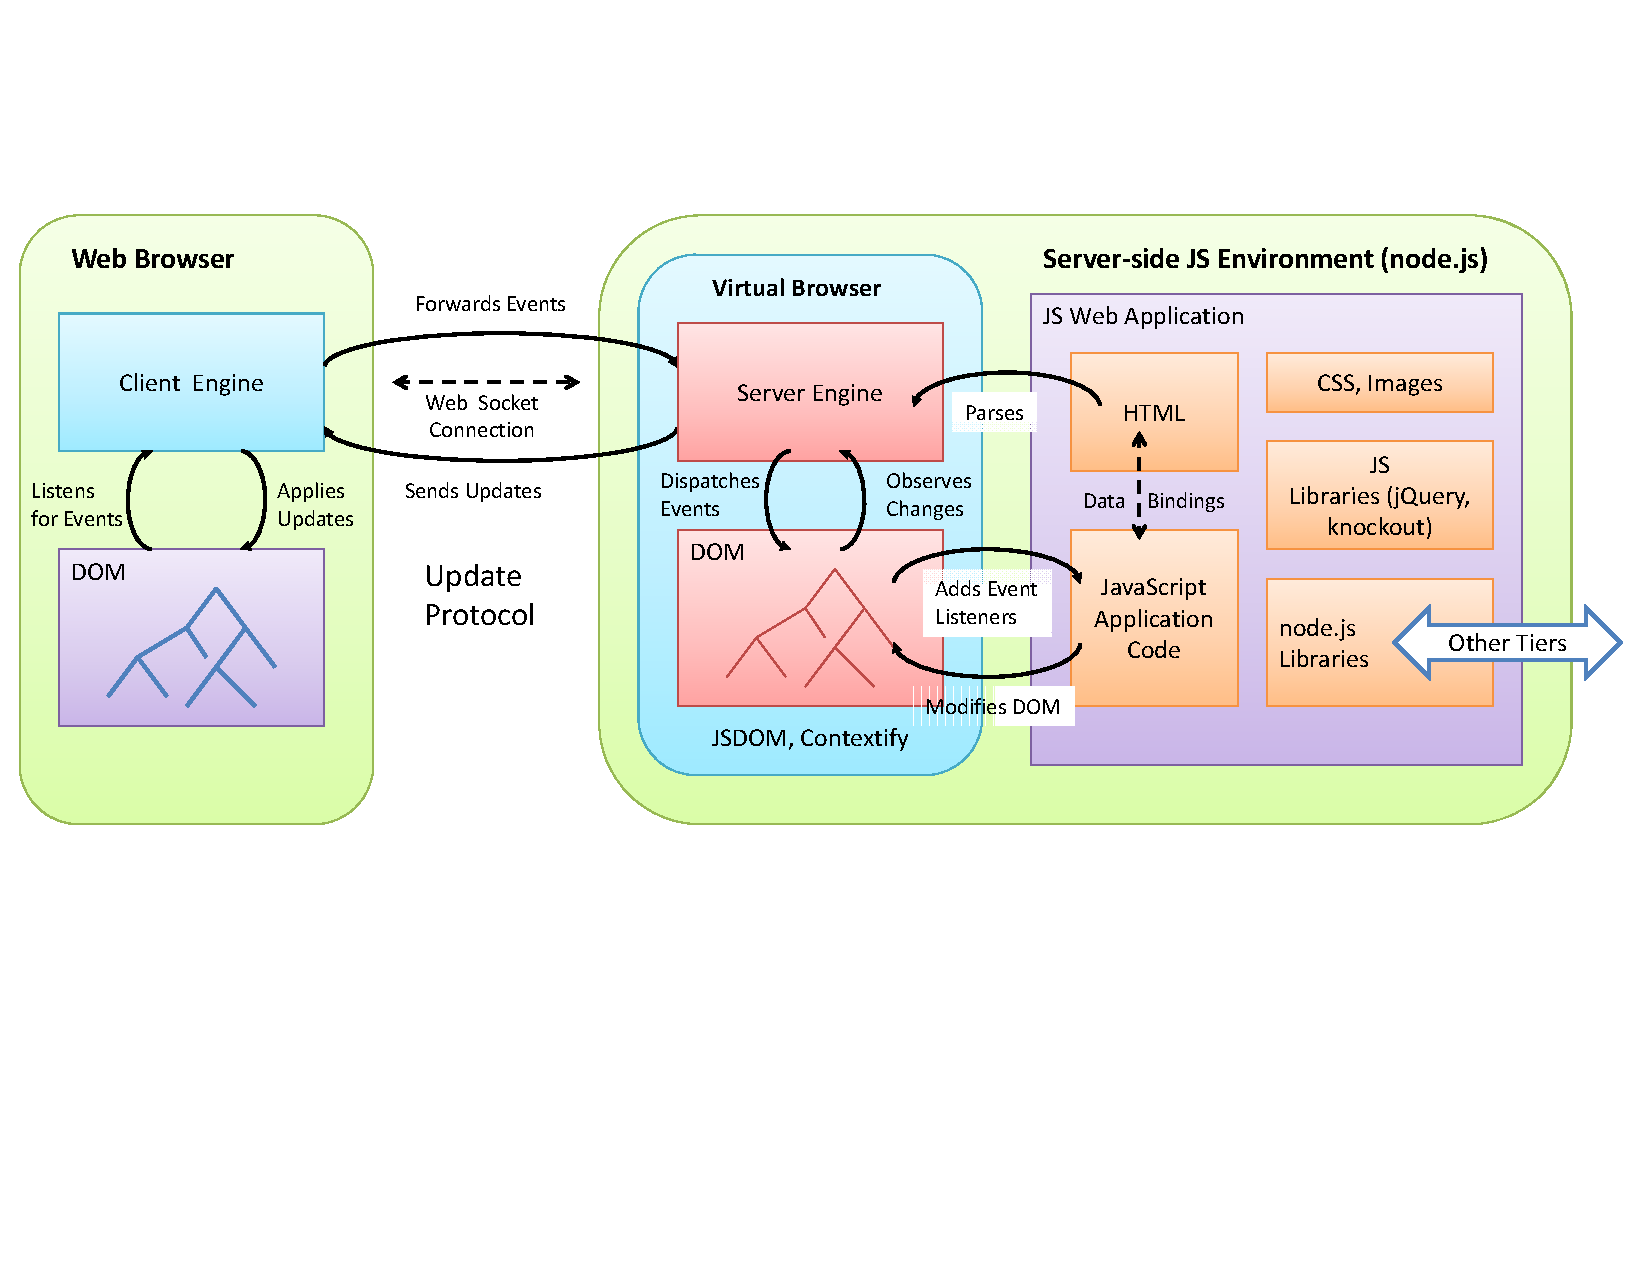
\includegraphics[width=\textwidth]{../figs/architecture_overview}
    \caption{Single Process \cb{} Architecture Overview}
    \label{fig:cb1arch}
    \end{figure*}
}

\newcommand{\newarchitectureoverview}{
    \begin{figure*}[ht]
    \centering
    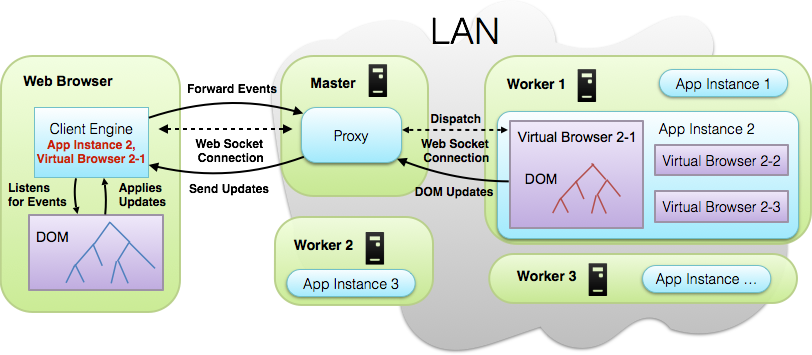
\includegraphics[width=\textwidth]{../figs/new_architecture_overview}
    \caption{Multiprocess Process \cb{} Architecture Overview}
    \label{fig:cb2arch}
    \end{figure*}
}

\newcommand{\requestdispatchdiagram}{
    \begin{figure}[ht]
    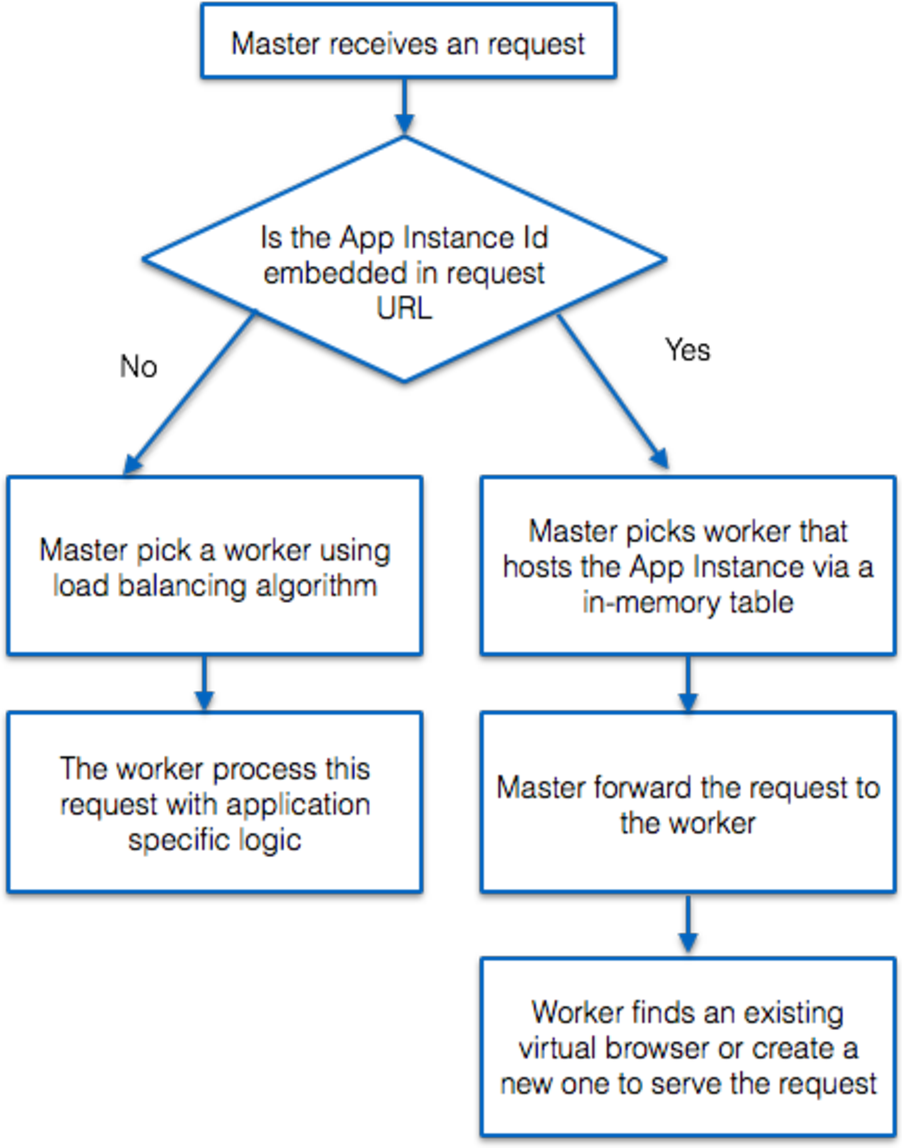
\includegraphics[width=0.4\textwidth]{../figs/request_dispatch}
    \caption{Request Dispatch Diagram}
    \label{fig:dispatch}
    \end{figure}
}

\newcommand{\appinstancefig}{
    \begin{figure}[ht]
    \centering
    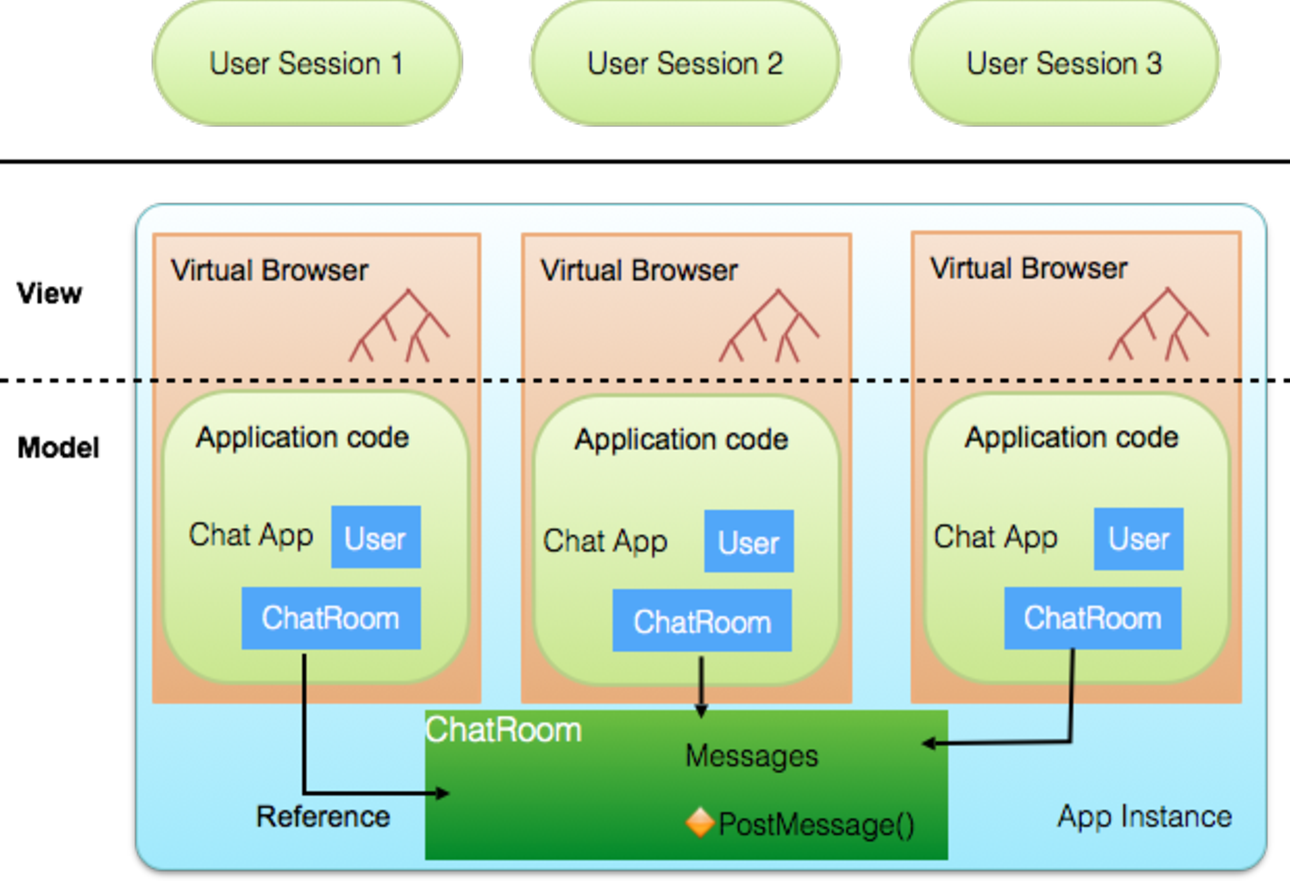
\includegraphics[width=0.5\textwidth]{../figs/appInstance}
    \caption{Detailed view of an App Instance}
    \label{fig:appinstance}
    \end{figure}
}


\newcommand{\chatappfig}{
    \begin{figure}[ht]
    \centering
    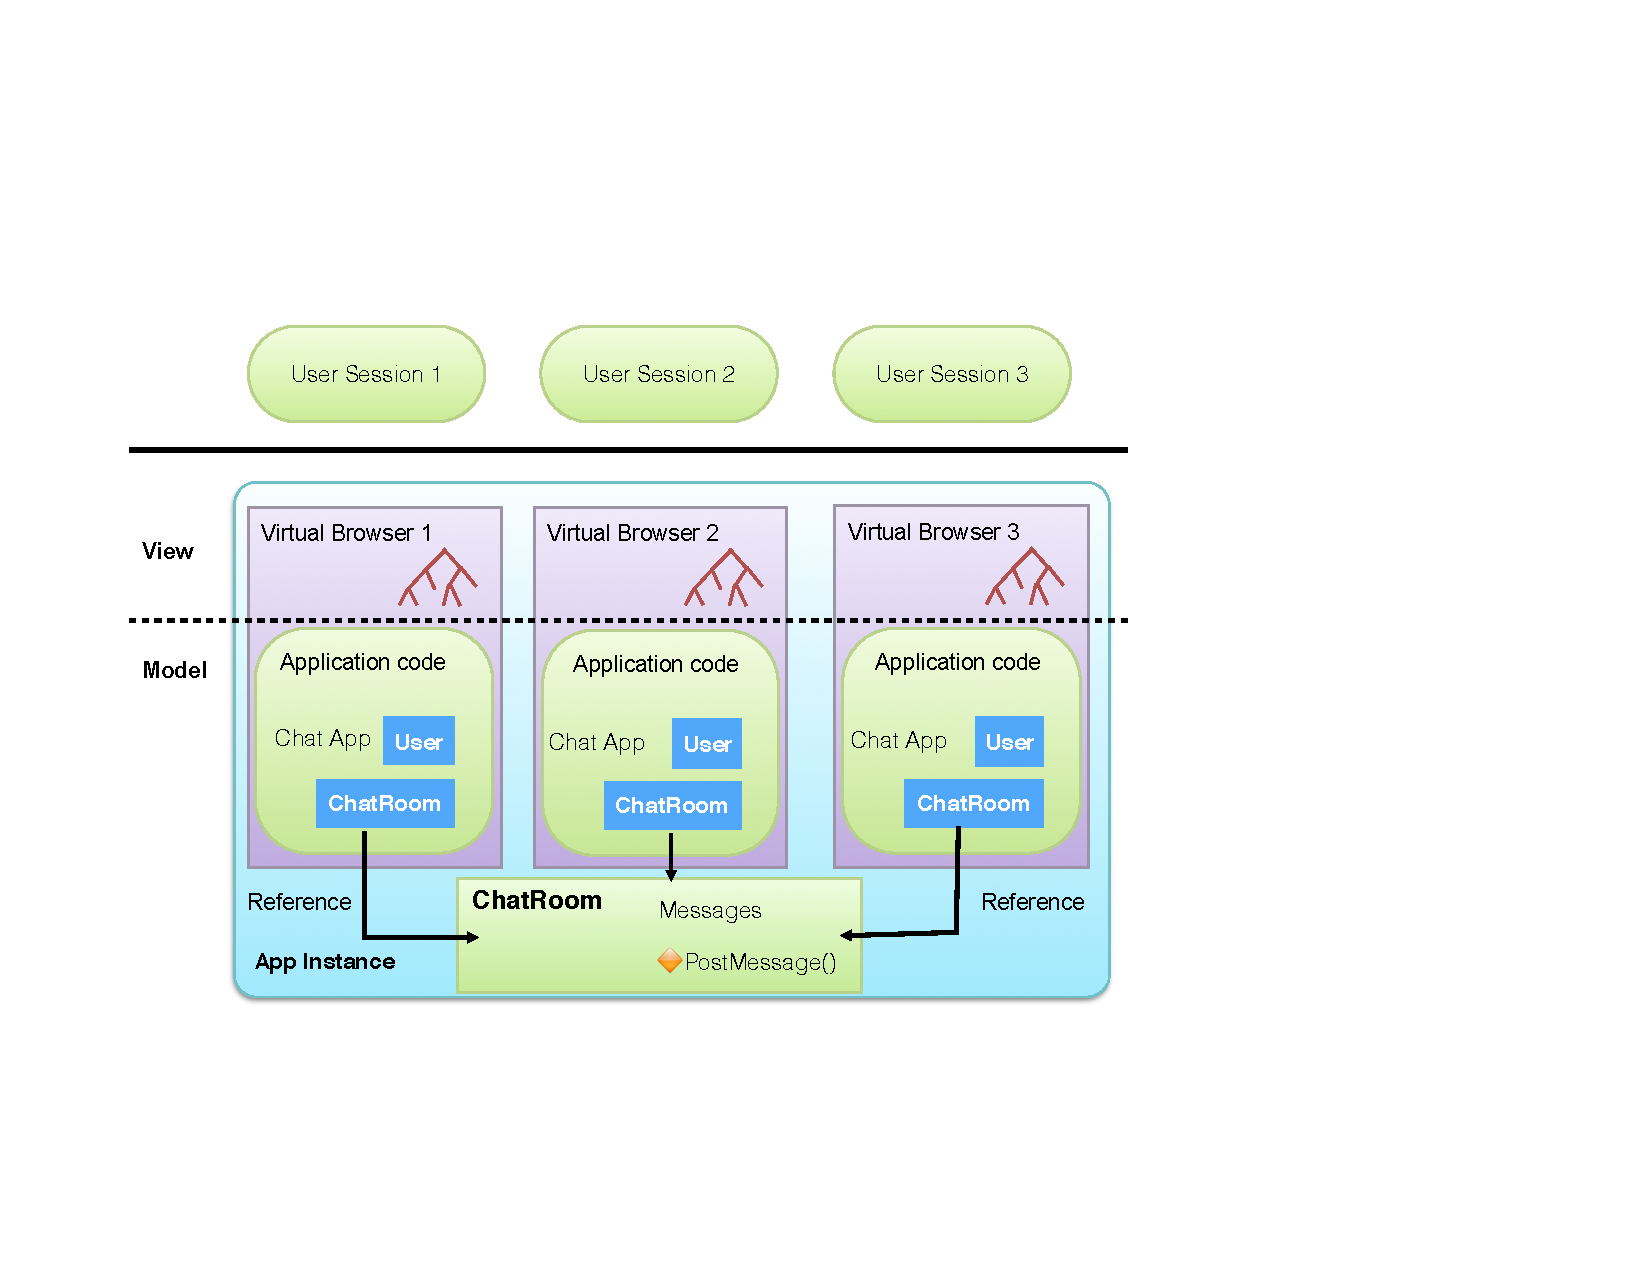
\includegraphics[width=0.5\textwidth]{../figs/chat_application}
    \caption{This figure shows how multiple virtual browsers can directly,
        and seamlessly share relevant application data, in this case chat messages,
        which then become part of the model that drives the presentation
        MVC framework.
    }
    \label{fig:chatapp}
    \end{figure}
}


\newcommand{\clickthroughput}{
    \begin{figure}[ht]
    \centering
    \includegraphics[width=0.5\textwidth]{../gnuplot/click_throughput}
    \caption{Throughput of ``Back-to-back'' click application.}
    \label{fig:clickthroughput}
    \end{figure}
}


\newcommand{\clicklatency}{
    \begin{figure}[ht]
    \centering
    \includegraphics[width=0.5\textwidth]{../gnuplot/click_latency}
    \caption{Latency of ``Back-to-back'' click application.}
    \label{fig:clicklatency}
    \end{figure}
}


\newcommand{\clickwaitthroughput}{
    \begin{figure}[ht]
    \centering
    \includegraphics[width=0.5\textwidth]{../gnuplot/click_wait_throughput}
    \caption{Throughput of click application, after introducing artificial delay.}
    \label{fig:clickwaitthroughput}
    \end{figure}
}


\newcommand{\clickwaitlatency}{
    \begin{figure}[tb]
    \centering
    \includegraphics[width=0.5\textwidth]{../gnuplot/click_wait_latency}
    \caption{Latency of click application, after introducing artificial delay.}
    \label{fig:clickwaitlatency}
    \end{figure}
}



\newcommand{\angularchatlatency}{
    \begin{figure}[tb]
    \centering
    \includegraphics[width=0.5\textwidth]{../gnuplot/angularchat_latency}
    \caption{Latency of chat application with Angular.js.}
    \label{fig:angularchatlatency}
    \end{figure}
}


\newcommand{\jquerychatlatency}{
    \begin{figure}[tb]
    \centering
    \includegraphics[width=0.5\textwidth]{../gnuplot/jquerychat_latency}
    \caption{Latency of chat application with JQuery.}
    \label{fig:jquerychatlatency}
    \end{figure}
}


\newcommand{\chatroomfig}{
    \begin{figure}[tb]
    \centering
    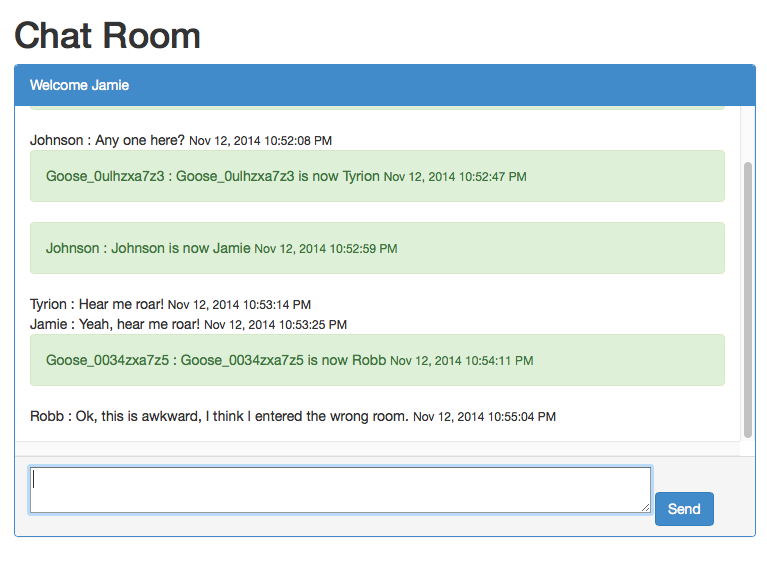
\includegraphics[width=0.5\textwidth]{../figs/chatroom}
    \caption{Chat Room Application}
    \label{fig:chatroom}
    \end{figure}
}

\newcommand{\apphierarchyfig}{
    \begin{figure}[tb]
    \centering
    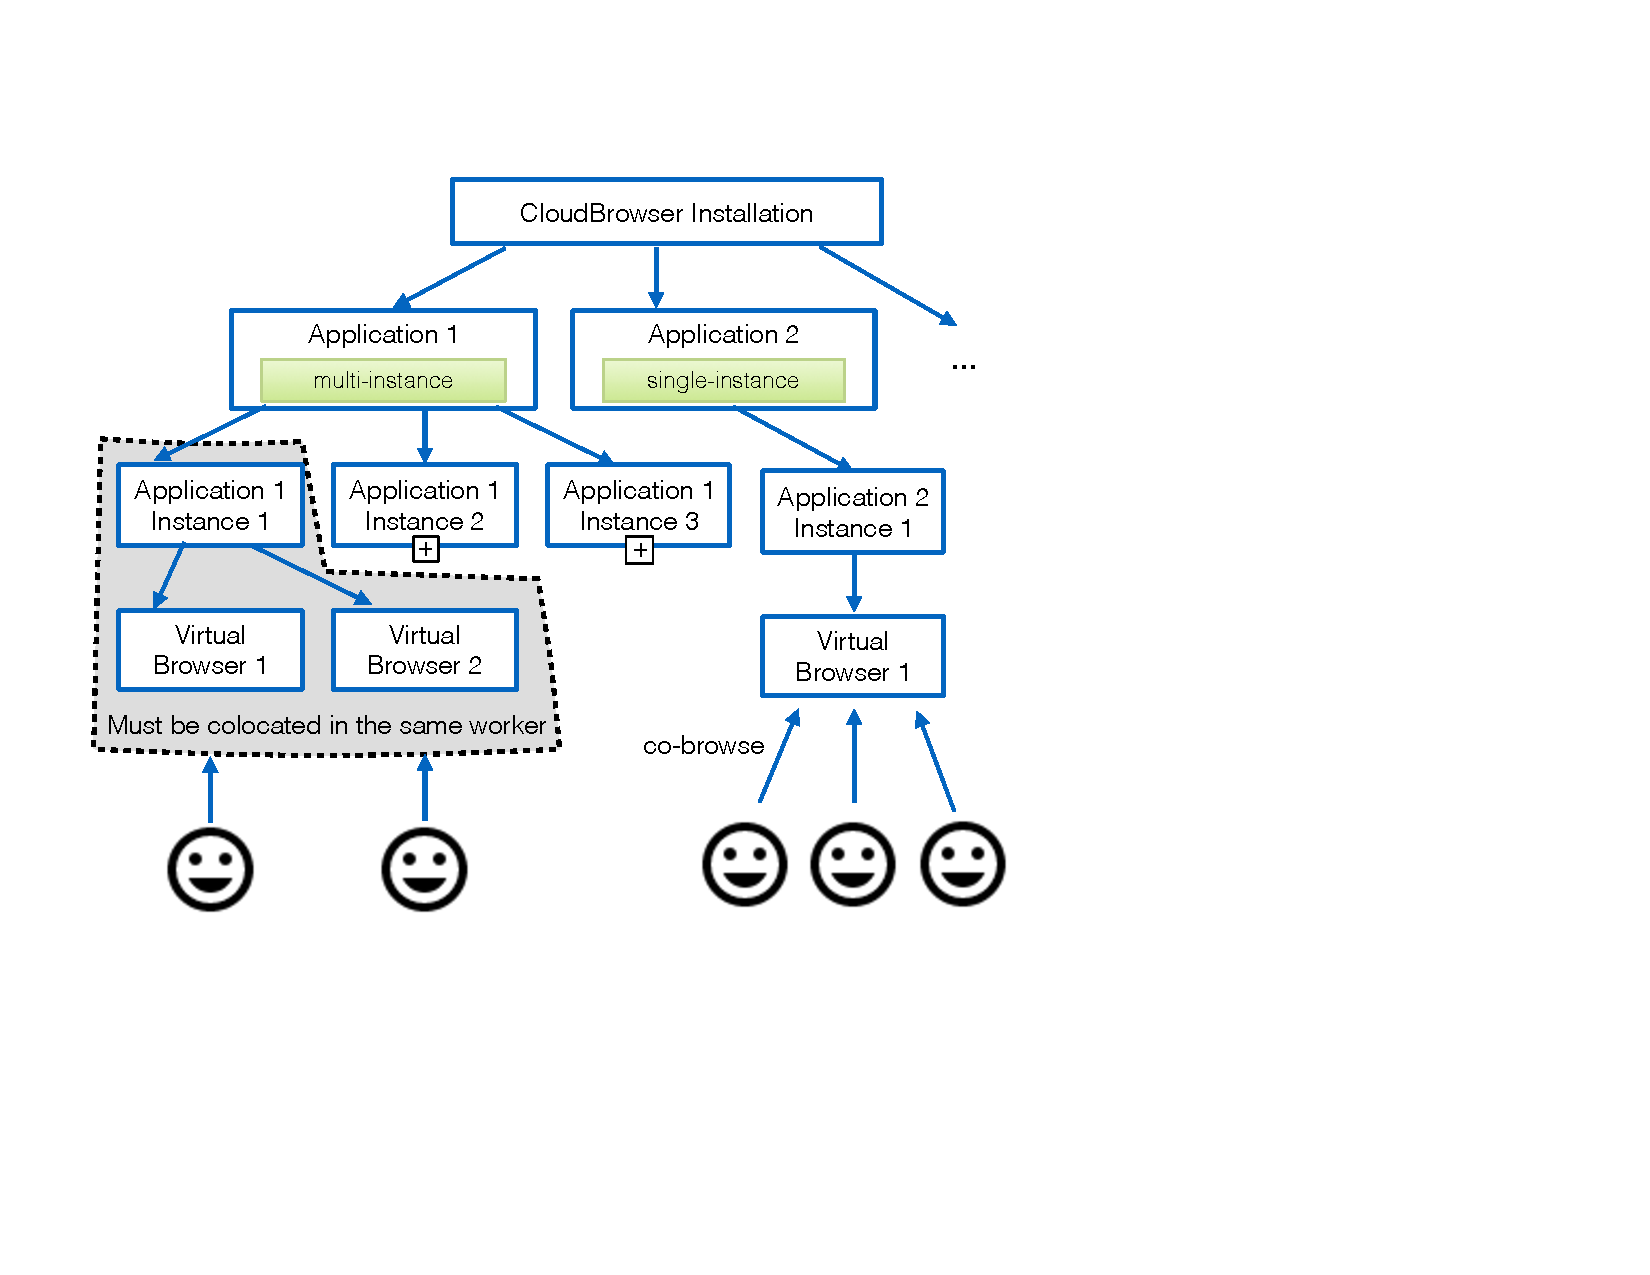
\includegraphics[width=0.5\textwidth]{../figs/application_hierarchy}
    \caption{Hierarchy of applications, application instances, and virtual browsers.
    Note that a single virtual browser may be broadcast to multiple clients (cobrowsing).}
    \label{fig:appidhierarchy}
    \end{figure}
}

\newcommand{\memfig}{
\begin{figure*}[ht]
    \centering
    \includegraphics[width=\textwidth]{../gnuplot/resource_consumption}
    \caption{
    Resource Consumption of worker node running JQueryChat Application\\
X axis is time. Left Y axis corresponds to the red line of CPU usage.
Right Y axis corresponds to memory statistics.\\
After about 90s after the system boots up, the benchmark tool starts to simulate 
user workload.
When the benchmark tool sending requests, \emph{HeapUsed} fluctuates as the system creates new objects and garbage collector cleans dead objects.
When the \emph{HeapUsed} drops there is a steep surge of CPU usage, indicating garbage collector is working at that time.
    }
    \label{fig:mem}
\end{figure*}
}


\newcommand{\nodermifig}{
    \begin{figure}[ht]
    \centering
    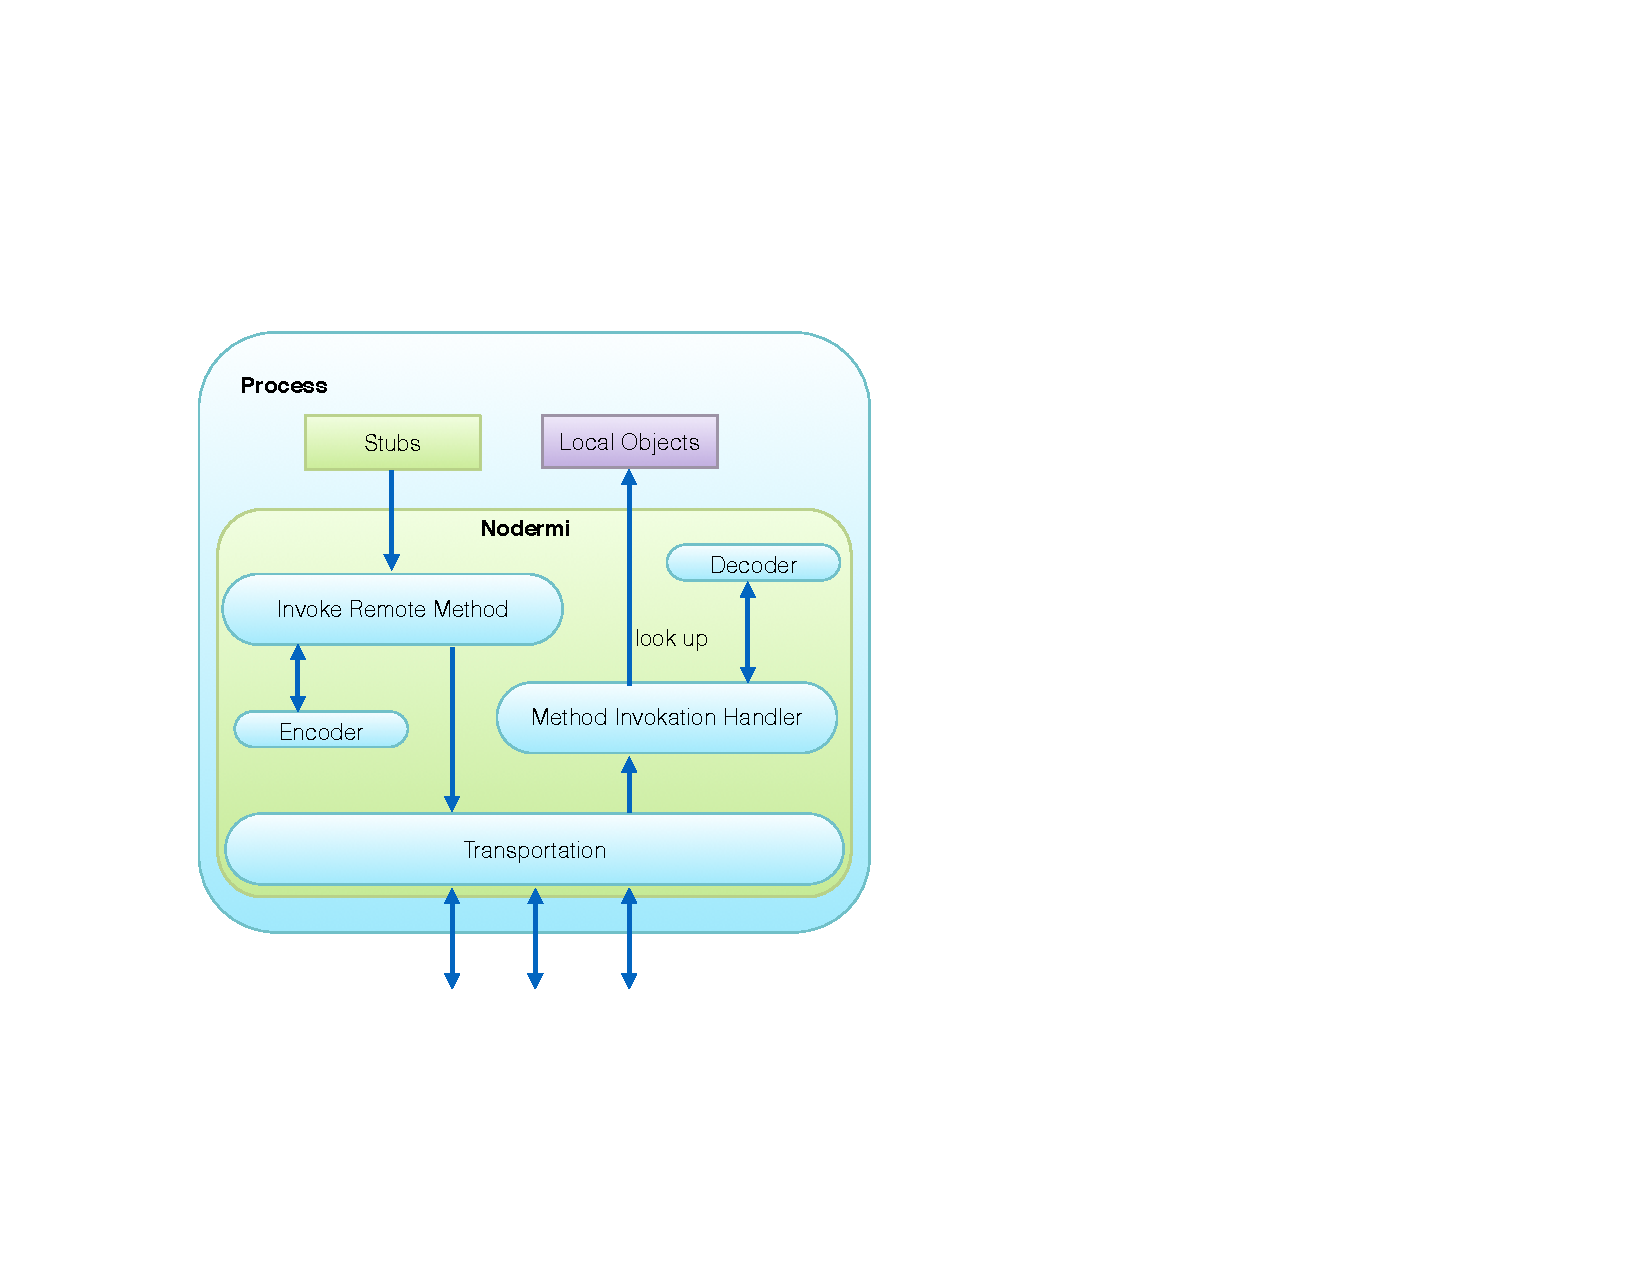
\includegraphics[width=0.5\textwidth]{../figs/nodermi}
    \caption{Overall Design of nodermi}
    \label{fig:nodermi}
    \end{figure}
}


\newcommand{\nodrmimethodinvokefig}{
    \begin{figure}[ht]
    \centering
    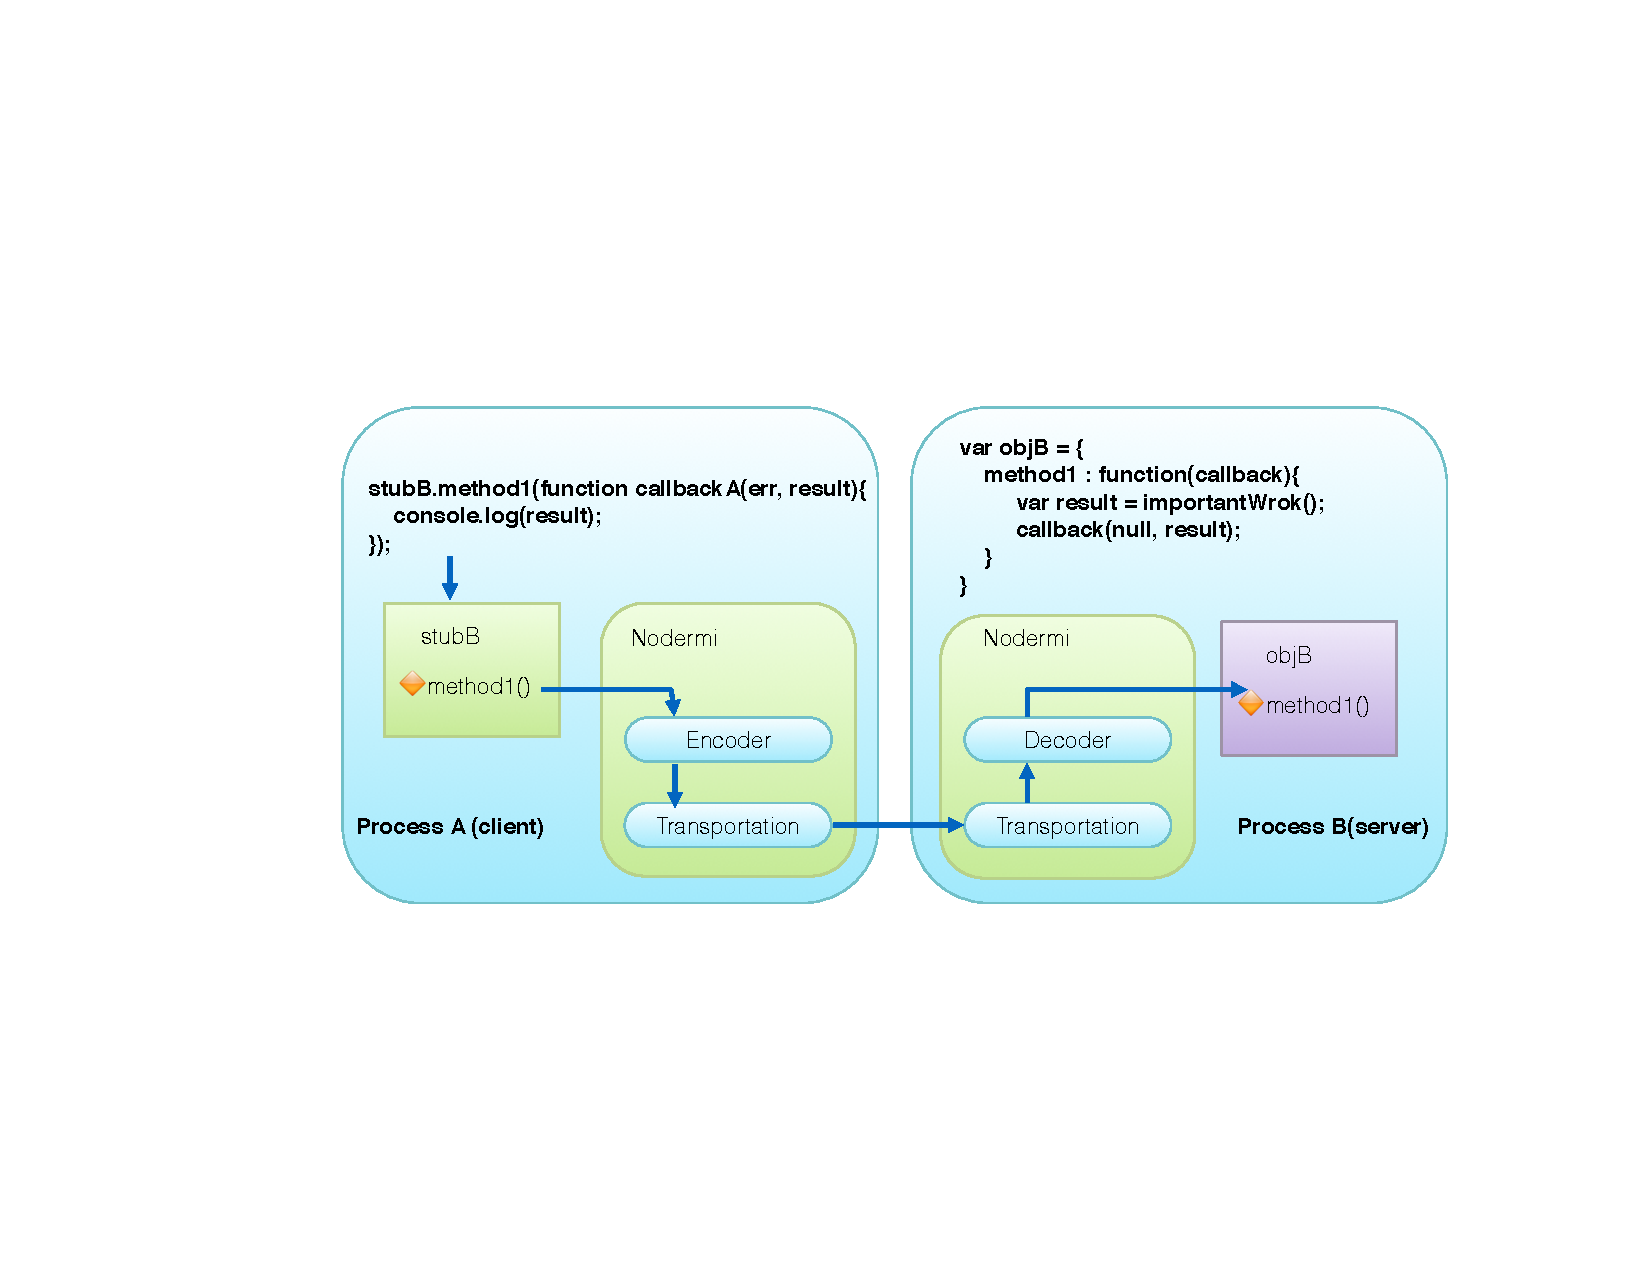
\includegraphics[width=0.8\textwidth]{../figs/nodermi_method_invoke}
    \caption{Process A invoke a method of a stub object}
    \label{fig:nodermimethodinvoke}
    \end{figure}
}


\newcommand{\nodrmicallbackfig}{
    \begin{figure}[ht]
    \centering
    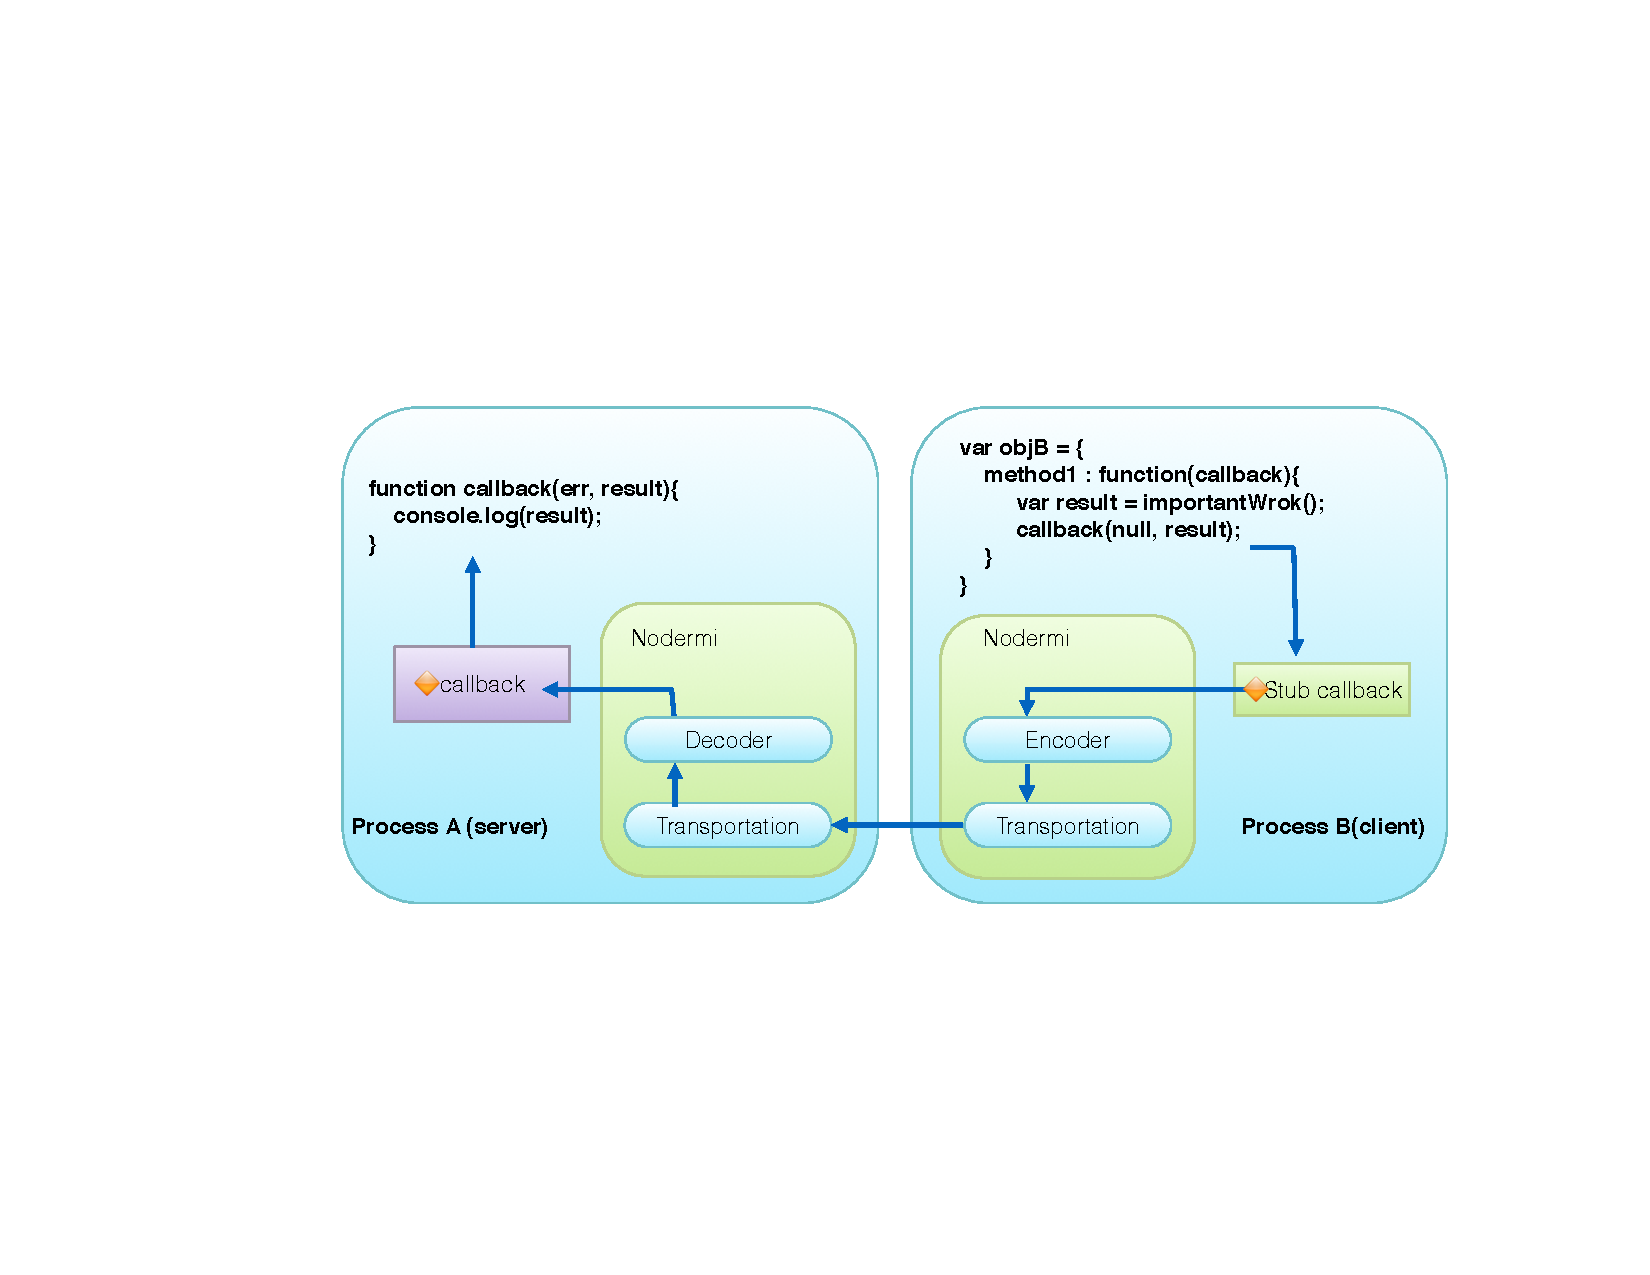
\includegraphics[width=0.8\textwidth]{../figs/nodermi_callback}
    \caption{Process B invoke a method that itself is a stub}
    \label{fig:nodermicallback}
    \end{figure}
}

\newcommand{\nodrmiobjmapfig}{
    \begin{figure}[ht]
    \centering
    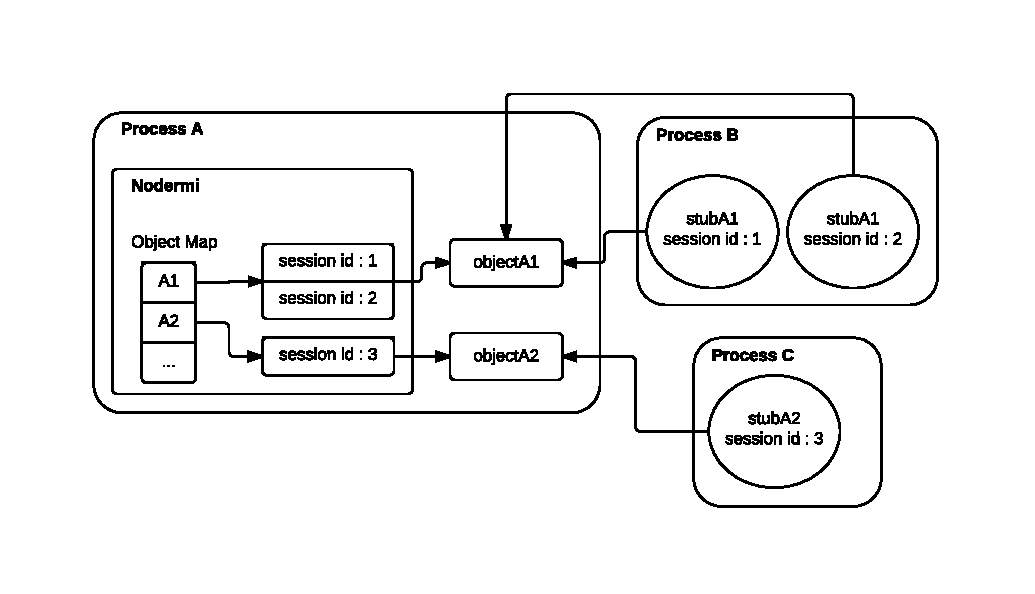
\includegraphics[width=0.8\textwidth]{../figs/nodermi_objectmap}
    \caption{Nodermi object map and stub map}
    \label{fig:nodermiobjmap}
    \end{figure}
}

\newcommand{\nodrmiracefig}{
    \begin{figure}[ht]
    \centering
    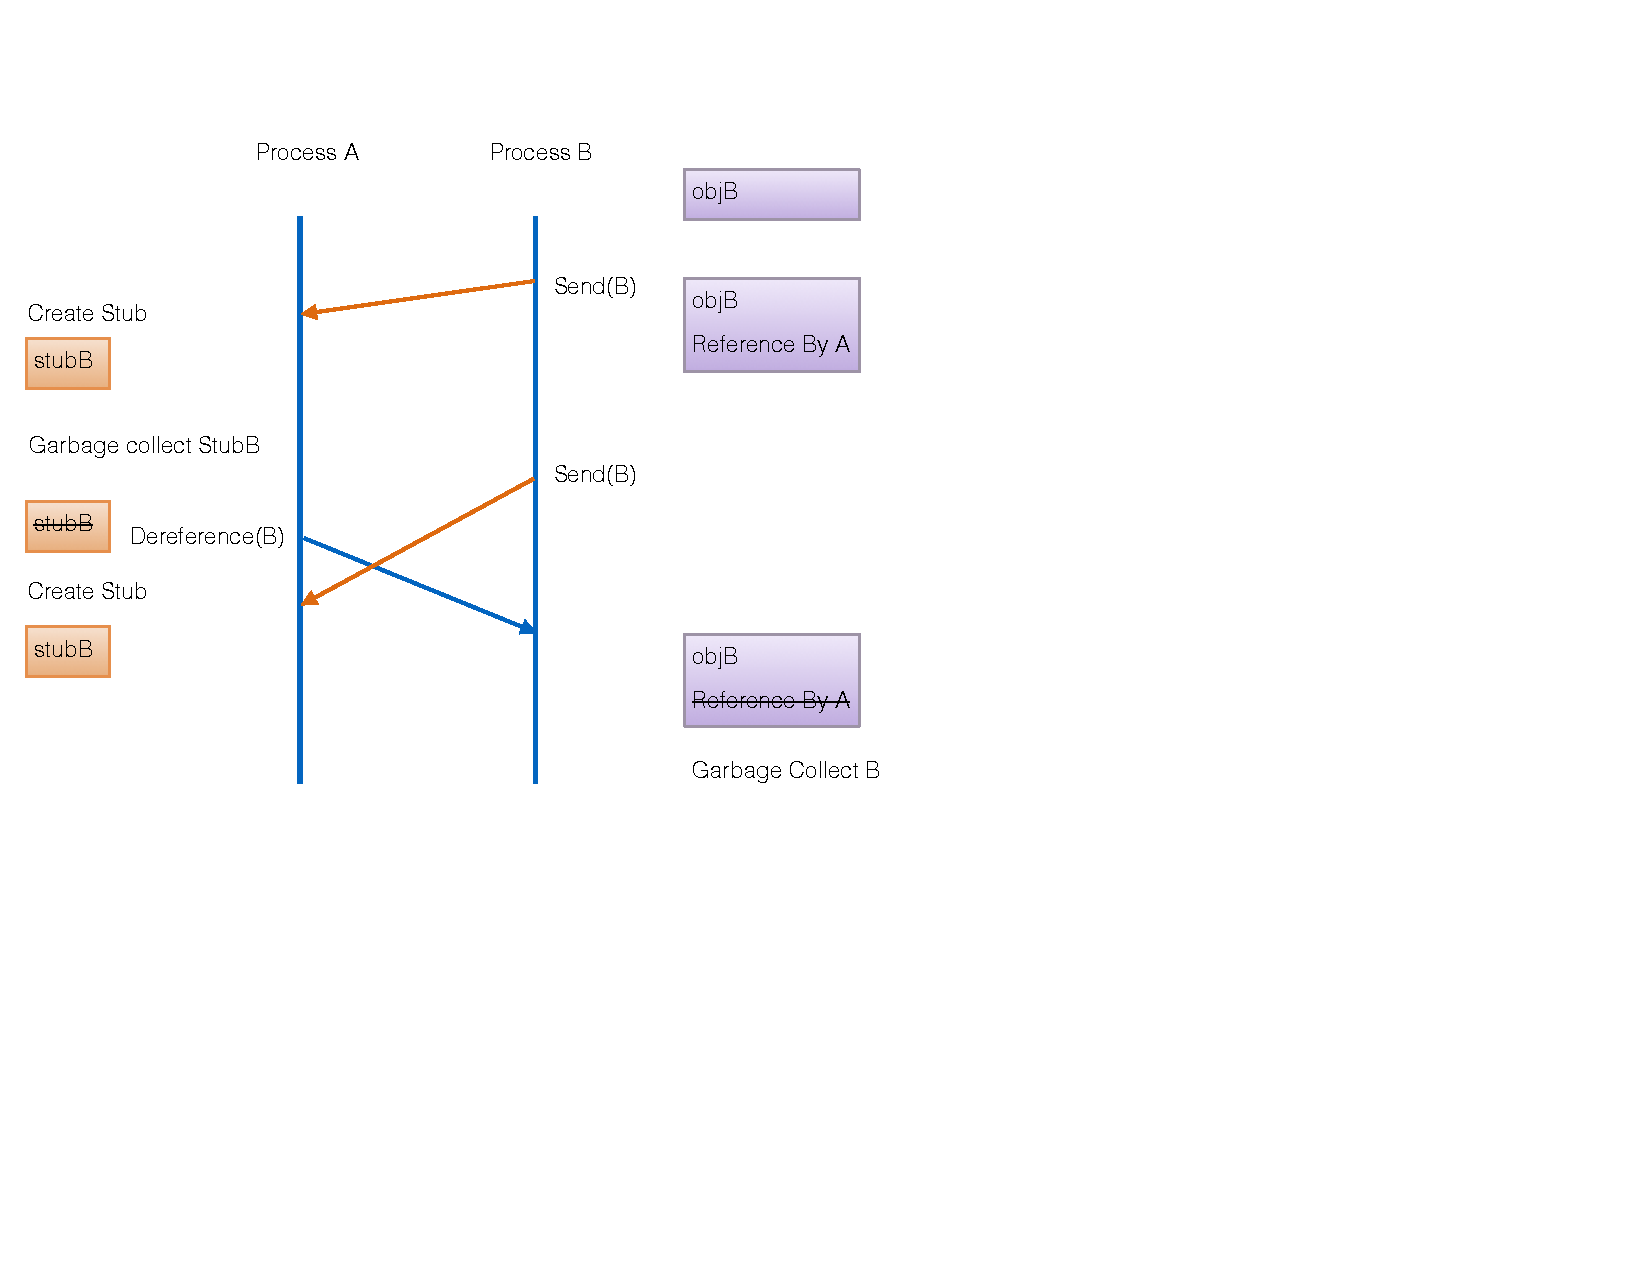
\includegraphics[width=0.8\textwidth]{../figs/nodermi_race}
    \caption{Race in dereference remote reference}
    \label{fig:nodermirace}
    \end{figure}
}
